\section{Transformation}\label{sec:trans}
Each component in Arcadia that we mentioned in the above section is to be translated into counterpart in AADL (e.g., functional block, port, connection, physical node). Since our approach focuses on generating AADL models for further analysis, during the transformation procedure, we theoretically neglect all the Arcadia attributes or parts of the components that exist only in Arcadia but could not find the corresponding object in AADL. On the other hand, some of the missing components and attributes in Arcadia are complemented when translated to AADL. This section presents the translation rules and the operation. In the following parts of the paper, several symbols are defined for the convenience of formal description of transformation rules (see table \ref{tab:symbol}), in which: one rule beginning from $\Gamma$ and end with ";"; the parent node is enclosed within the angle brackets "< >" (if it has one parent node); the attribute group are enclosed with parentheses "\{ \}"; square braces "[ ]" delimit optional elements and the alternatives are separated by a pipe "|"; each part of object separated by ":"; and the parentheses with plus "\{ \}+" is used to present the option is to be created; for some ignored attributes and objects are donated "$\neg$" which is in front of ignored object. An example of transformation rule expressions is in listing \ref{code:T_port}. What we have to note is each rule can contain one source object which in the left of transfer symbol $\rightsquigarrow$ and one or more attributes, and in the right side is target object and its member attributes. In particular, the number of attributes of the target object may be greater than the number of attributes of the source object in the case of a new object created.%\multimap$

\input{codes/ha.aadl}

%%--------------表格
\begin{table}[h] 
\centering
\normalsize
\begin{tabular}{lr}
\hline
\textbf{Symbol} & \textbf{Meaning} \\ \hline 
$\Gamma$ & Transformation Rule \\ 
; & End of rule \\ 
$\rightsquigarrow$ & Transfer \\
\textless \textgreater{} & Parent node \\ 
\{ \} & Attribute \\ 
{[} {]} & Optional element \\ 
| & Separation of elements  \\
\{ \}+ & Attribute is to be created \\ 
$\neg$ & Ignore \\ \hline
\end{tabular}
\vskip 0.5cm
\caption{Symbols of transformation rule expression}
\label{tab:symbol}
\end{table}

%%-------------------------------



\subsection{Port and Connection}
Ports are the logical connection points between components. AADL defines three types of component ports, for the transmission of data by data port, control information by event port and both of them by data event port. There are two directions of port, input, and output. The output port is connected to the input port to constitute the port connection. On the other hand, Arcadia defines only directions (in and out), the type of port is omitted. Hence, we ought to add the type attribute to complete the form in AADL when doing a transformer. The translating rule writes as an example in list \ref{code:T_port} at line 1. It means the transformation of one functional port $P_{ort}$ of Arcadia to a port of AADL (within the parent node \textit{<feature>}). The direction attribute and its values \textit{in or out} can transfer to counterpart directly, and the data type is additional option, it will be add with its values \textit{data, event, data event}, denoted~\textit{\{Type[data|event|data event]\}+}. For some attribute which does not exist in AADL such as \textit{ordering} (see list at line 3), we can write one line with the symbol $\neg$, it means the ordering attribute will be ignored for transformation. 

A connection is an interaction between two objects via ports. One connection must have only one \textit{source} and \textit{target}. It is the same in both Arcadia and AADL. An example of transformation expression is shown in line 4. 

However, all the transformation rule expression depends on the needs of engineering, if designers need some of the attributes to carry out analysis in next steps, they can add that they need, otherwise, they can write one line of expression to declare to ignore or omit it. 


%%--------------代码
\begin{lstlisting}[caption={An example of transformation rules}, label=code:T_port,mathescape=true]
$\Gamma$$P_{ort}$:{Direction[in|out]})$\rightsquigarrow$ <feature>:Port:{Direction[in|out]}:{Type[data|event|data event]}+;
$\Gamma PP \rightsquigarrow$ <feature>:Port:{Direction[in|out]}+:{Type[data|event|data event]}+;
$\Gamma P_{ort}$:$\neg${ordering});
$\Gamma Ex_{fun}$:{Source}:{Target} $\rightsquigarrow$ <connections>:connection:{source}:{target}; 
\end{lstlisting}
%%-------------------------------

\subsection{Logical components}
%%--------------表格 功能转换
\begin{table*}[h]
\resizebox{\textwidth}{!}{%
\begin{tabular}{lll}
\hline
\textbf{Arcadia} & \textbf{AADL} & \textbf{Additional attributes} \\ \hline
logical component container ($C_{omp}$) & process, system & \{Runtime\_Protection{[}true|false{]}\}+ \\
functional port container ($FPC$) & feature group & $\bigcirc$ \\
port allocation ($P_{alloc}$) & binding & $\bigcirc$ \\
exchange of logical component ($Ex_{comp}$) & binding & $\bigcirc$ \\
function ($F_{un}$) & thread, abstract & \{Dispatch\_Protocol{[}Periodic|Aperiodic|Sporadic|Background|Timed|Hybrid{]}\}+ \\
port ($P_{ort}$) & port & \{Type{[}data|event|data event{]}\}+ \\
exchange of function & connection & $\bigcirc$ \\
allocation & binding & $\bigcirc$ \\ \hline
\end{tabular}%
}
\vskip 0.5cm
\caption{Functional elements corresponding table}
\label{tab:funcionalT}
\end{table*}
%%-------------------------------

The logical components in Arcadia contain a set of member elements, such as logical component containers, functions, ports, and functional exchanges. In order to find the counterpart in AADL, we give an explicit correspondence table according to metamodels of Arcadia and AADL (see the formal definition of the logical component of Arcadia \ref{def:lc} and formal definition of software functional composition in AADL \ref{def:sfc}). In other words, the designer can combine the functional subset of Arcadia with the software functional composition subset of AADL using their metamodels. 




\subsection{physical component}
The physical component in Arcadia consists of physical Node, Port and Link. The Physical Port and Link correspond to port and bus connection in AADL. There are some choices when the physical Node is translated to AADL such as device, memory, and processor, hence the designer has to point out what type of target component during transformation by using transformation rule express. The table \ref{tab:PhysicalT} given an example of the corresponding relation of the physical component between Arcadia and AADL.
%%--------------表格 物理组件转换
\begin{table*}[h]
\resizebox{\textwidth}{!}{%
\begin{tabular}{lll}
\hline
\textbf{Arcadia} & \textbf{AADL} & \textbf{Additional attributes} \\ \hline
physical component ($N_{ode}$) & device,memory,processor & \{Dispatch\_Protocol\}+:\{Period\}:\{Deadline\}+:\{priority\}+ \\
physical component port ($PP$) & port & $\bigcirc$ \\
exchange of logical port and physical port ($Ex_{fpp}$) & binding & $\bigcirc$ \\
physical link ($PL$) & bus & $\bigcirc$ \\ \hline
\end{tabular}%
}
\vskip 0.5cm
\caption{Physical elements corresponding table}
\label{tab:PhysicalT}
\end{table*}
%%-------------------------------


\subsection{Hybrid Annex}
When transforming the behavioral description to a Hybrid annex, one must provide some necessary elements like variables, invariants, constants, channels, and behavior. Since Hybrid annex adopts the process algebra notations, the behavior of components is described by a set of CPS process; mostly it uses the differential equation for a continuous process. For example, the acceleration and deceleration in the traction control system of the train, refer to listing \ref{code:aadl}. 

During the transformation, the continuous evolution of a CPS processes is expressed by some differential equations, which would be an attribute of the functional component in Arcadia. As an example shown in Listing \ref{code:aadl}, the differential expression 'DT 1 m*dv/(P-Q-m*g*$\alpha$)' describes the relationship between distance and acceleration time, where m is mass of train, P is the tractive effort of the locomotive, Q is the drag in Newton, alpha is the gradient. the differential equation is written as \[m\frac{dv}{dt}=P(v)-Q(v)-mg\alpha\] 
which, once the initial speed is given, defines $v$ as a function of time $t$. For the deceleration is the same, one just considered time the breaking factor. 
However, there are still some correlated variables are not declared in Arcadia, in this case, the designer has to add (create) them in Hybrid Annex code. 

\begin{lstlisting}[caption={Translating of Hybrid Annex},label=code:ha,mathescape=true]
$\Gamma [F_{un}|C_{omp}]$:equations $\rightsquigarrow$ <[abstract|system|process|thread]>:<hybrid annex>:behavior;
$\Gamma [F_{un}|C_{omp}]$ $\rightsquigarrow$ <[abstract|system|process|thread]>:<hybrid annex>:{assert}+:{invariant}+:{variables}+:{constants}+;
\end{lstlisting}



\subsection{Implementation of Arcadia2AADL transformation tool}

\begin{figure}[!hbt]
\centering
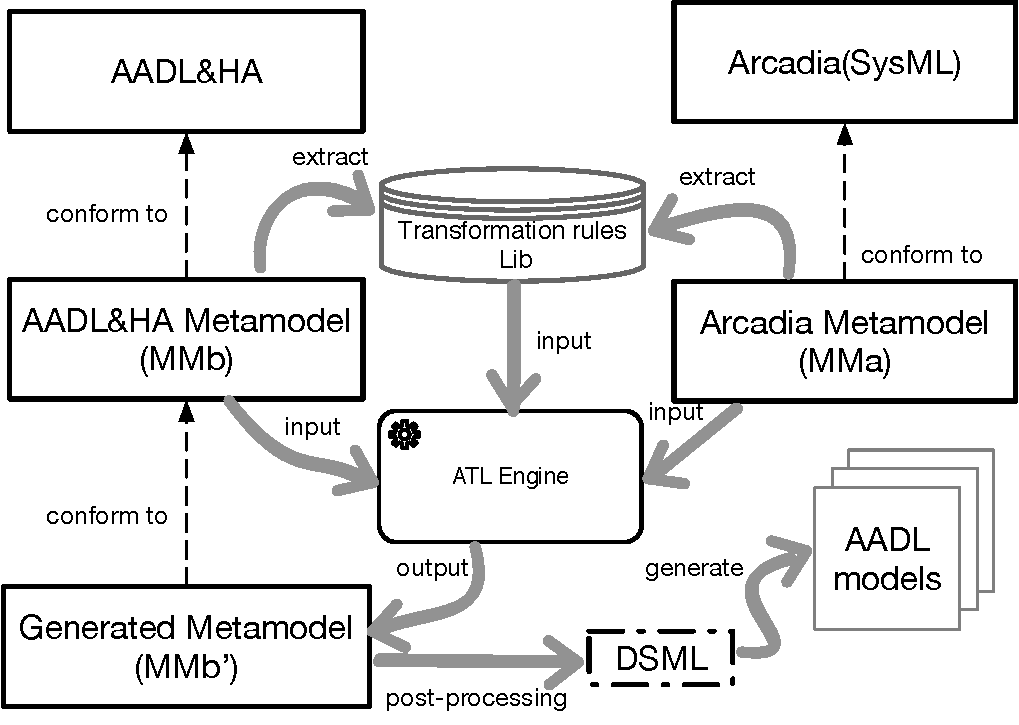
\includegraphics[width=.95\linewidth]{img/transfer_workflow}
\caption{Structure of Arcadia2AADL model transformation tools}
\label{fig:twf}
\end{figure}

Based on the translation rules defined in section \ref{sec:trans}, we implemented Arcadia2AADL transformation tool which can generate target metamodel according to original metamodels and transformation rule library. The ATL serves as a transformation engine. For more detailed information of ATL, the reader is referred to~\cite{Jouault:2006ft}\cite{Jouault:2008bz}. 
The tool architecture is shown in Fig \ref{fig:twf}. AADL\&HA (denoted as MMb) and Arcadia metamodels (denoted as MMa) are imported (input) into ATL engine and the engine is going to read transformation rules library and then the transformation engine exports (output) the corresponding metamodel (denoted as generated metamodel MMb') which is a subset of AADL\&HA, in other words, the generated metamodel is fit AADL and its hybrid annex. The generated metamodel is then further post-processed as a DSML (domain-specific modeling language) in \textit{ecore} format. Which can be used to create concrete models. Therefore, all concrete models afterward are conformed to this metamodel and will be used for further verification and analysis.  
